\documentclass[12pt]{article}
\usepackage{verbatim}
\usepackage[left=1in,right=1in,top=1in,bottom=1in]{geometry}
\usepackage{color}
\usepackage{xcolor}
\usepackage{nicefrac}
\usepackage{xfrac}
\usepackage{bm}
\usepackage{mathtools}
\usepackage{amssymb}
\usepackage{cancel}
\usepackage{enumerate}
\usepackage{amsthm}
\usepackage{graphicx}
\usepackage{tocloft}
\usepackage{setspace}
\usepackage{marginnote}
\usepackage{ulem}
\usepackage[perpage]{footmisc}
\usepackage{fontspec}
\usepackage{microtype}
\usepackage{listings}
\usepackage{adjustbox}
\usepackage[mmddyyyy]{datetime}
\usepackage{amsmath}
\usepackage{unicode-math}
\usepackage{titlesec}
\interfootnotelinepenalty=10000
\hbadness=350
\tolerance=7000
\pretolerance=1500
\relpenalty=9999
\binoppenalty=9999
\emergencystretch=0pt
\righthyphenmin=4
\lefthyphenmin=4
% \titleformat{\section}{\filcenter\normalfont\Large\bfseries}
% {\MakeUppercase{\chaptertitlename}~\thechapter:} {0.5em} {}
% \titlespacing{\chapter}{0pt}{0pt}{10pt}
\defaultfontfeatures{Ligatures=TeX}
\setmathfont{XITS Math}
\graphicspath{{images/}}
\definecolor{mytext}{HTML}{000000}
\usepackage[hang]{caption}      % to indent subsequent lines of captions
\renewcommand{\captionfont}{\bfseries} % bold caption (needed with caption 
                                       % package to restore boldface.)
                                       % \includeonly{app}
\pagestyle{plain}
\renewcommand{\contentsname}{\centerline{\huge{\textbf{\textup{MASTER PLAN}}}}}
\setlength\parindent{2.5em}
\mathtoolsset{showonlyrefs,showmanualtags}
\renewcommand{\thefootnote}{\fnsymbol{footnote}}
\usepackage[nottoc,numbib]{tocbibind}
\usepackage[toc,indexonlyfirst,xindy]{glossaries}
\newglossarystyle{mylong3col}{%
  \setglossarystyle{long3colheader}%
  \renewcommand\entryname{Symbol}
  \renewcommand{\pagelistname}{First Use}
  \renewenvironment{theglossary}%
    {\setlength\LTleft{0pt}
     \setlength\LTright{0pt}
     \begin{longtable}[l]{@{}lp{0.675\textwidth}p{0.15\textwidth}}}%
    {\end{longtable}}%
    }
    \usepackage[hyphens]{url}
\usepackage[hidelinks,breaklinks,colorlinks=true,urlcolor=black,citecolor=mytext,linkcolor=mytext]{hyperref}
% \newglossary[isg]{issues}{iso}{isi}{List of Issues with Current Draft}
% \newglossary[slg]{symbols}{slo}{sli}{LIST OF SYMBOLS}
% \setglossarystyle{mylong3col}
% \setlength{\glsdescwidth}{0.675\textwidth}
\newcommand{\myj}{\mathscr{j}}
% \input{glossary}
\newcommand{\xs}{\gls*{boldx0}}
\newcommand{\x}{\gls*{boldx}}
\newcommand{\dfn}{\gls*{deltafn}}
\newcommand{\kron}{\gls*{kronecker}}
\newcommand{\dens}{\gls*{dens}}
\newcommand{\gi}{\gls*{gi}_i}
\makeatletter
\newcommand \Dotfill {\leavevmode \cleaders \hb@xt@ 0.8em{\hss .\hss }\hfill \kern \z@}
\makeatother
\renewcommand*\glspostdescription{\Dotfill}
\makeglossaries
\newcommand\numberthis{\addtocounter{equation}{1}\tag{\theequation}}
\numberwithin{equation}{section}
\setlength\cftsubsecnumwidth{4em}
\newcommand{\negphantom}[1]{\settowidth{\dimen0}{#1}\hspace*{-\dimen0}}
\renewcommand{\footnotesize}{\small}
\begin{document}
% \setlength\cftbeforechapskip{0pt}
\setlength{\cftbeforetoctitleskip}{9pt}
\setlength{\cftbeforeloftitleskip}{9pt}
% \renewcommand\cftchapleader{\cftdotfill{\cftdotsep}}
\urlstyle{tt}
\newtheorem{prop}{Proposition}
\newtheorem{theorem}{Theorem}
\newtheorem{lemma}{Lemma}
\newtheorem{corrolary}{Corrolary}
\newtheorem{defn}{Definition}
\begin{spacing}{1.15}

\tableofcontents
\pagebreak
\end{spacing}
\begin{spacing}{1.15}
\end{spacing}
\begin{spacing}{1.15}
\section{Introduction}
In this repository, we are developing code to solve a practice image classification problem that can be found at \url{https://datahack.analyticsvidhya.com/contest/practice-problem-identify-the-apparels}. Here, we document our data, our model, our code, our repository, and our plans for testing and for tuning parameters. 
\subsection{What this Document Still Needs}
This document is a work in progress. It needs quite a bit of editing and many more hyperlinks, and there are sections that have not been completed. We have not gone over the dense neural network model at all, nor have we discussed all of the parameters of the convolutional network. We also should switch to using bullet-pointed lists to discuss parameters rather than doing so in pure paragraph form, as we are doing at the moment. My attempts at visualizing the networks as graphs had to be postponed because of a prolonged and mostly unproductive fight with bugs in {\ttfamily keras.utils.plot\_model()}.

I wrote a script ({\ttfamily docs/scripts/find\_docstrings.py}) that extracts docstrings from all the functions in the {\ttfamily code/} directory, and the next project on that front is write another script to convert that documentation into a format that will look good in a LaTeX document. I hope to be able to use such scripts in this project and future projects to produce pdf documentation of my code that updates itself automatically.

The biggest missing piece is the unwritten section on testing strategy. While we touch on that when we discuss the parameters of our image processing and model design functions in \S\ref{imageprocessingparams} and \S\ref{convolutionalparams}, we need a fully organized plan for testing and tuning. The plan will be stored here, while documentation of the actual test runs will be in a separate pdf.

Beyond that, I want to add a section on optimizers. There are some facts that I gleaned from papers on that subject and a few others, so I also plan to add a bibliography. Glossaries are also generally useful, and we will add one.

\section{Data}
We begin by discussing our data. For now, we only use the 60000 training examples in the {\ttfamily train/} directory. Note that you must extract {\ttfamily train\_LbELtWX.zip} to obtain these examples, as the {\ttfamily train/} directory is deliberately omitted from the repository for performance reasons. These examples are images of 10 classes of apparel, with 6000 examples of each image. Each image is $28\times 28$ and grayscale. We plot some samples of each class in Figure \ref{fig:sampleimages}.

\begin{figure}
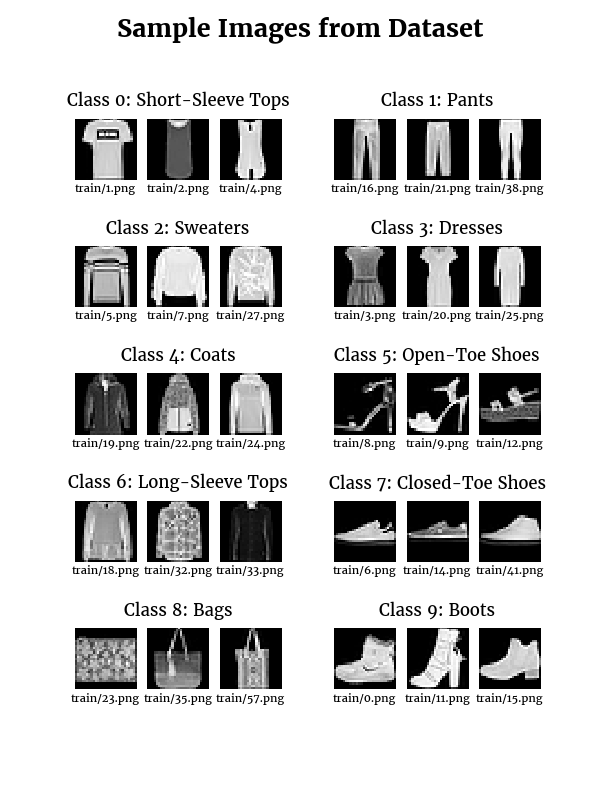
\includegraphics{sample_images.png}
\caption{We inspect 3 samples from each class of apparel, with predefined class numbers, class names as interpreted by the author, and source files.}
\label{fig:sampleimages}
\end{figure}
\subsection{Basic Analysis}
The dataset here is artificially clean: all the images are centered and upright, with nothing in the background. This should make it easier for our models to classify the data. It also means that some of the advantages of convolutional neural networks over dense neural networks may disappear; however, I still expect that a convolutional neural network will outperform a dense neural network, a belief that has been substantiated by the (undocumented) tests I have run up to this point. Nonetheless, I am training dense neural networks in addition to convolutional networks. I am not doing this because I expect great performance; rather, when I solve computer vision problems with ``messier'' data in the future, I would like to test the hypothesis that dense neural networks will be relatively less effective than in the case of this rather neat dataset.
\subsection{Loading the Data}
The module {\ttfamily load\_data} handles the process of importing data from the {\ttfamily train/} directory. It uses {\ttfamily matplotlib.pyplot.imread()} to load the data, only storing one channel in memory, as the images are grayscale. This will also make it easier to use the GitHub repository. In the future, we can make data loading faster by storing images in grayscale on the drive, preferably in one file; in the dataset, they came as RGB images with three identical channels. When we split the data into training and cross-validation sets in our training scripts, we always use 60\% of the images for training and a random seed of {\ttfamily 1}. Using the same random seed across all tests is critically important, as otherwise there would be no real distinction between our training and cross-validation data.

\subsection{Subdivision of the Classes}
We can see that our classes can be divided into several subgroups that are similar to each other. For example, sweaters and coats may be hard to distinguish, as may boots and close-toed shoes, but footwear can likely be distinguished from outerwear rather easily. While we can most likely get good performance without considering this aspect of our dataset, it may be that there is a way to exploit this concept to save computation time or improve accuracy.

I have not implemented or tested this idea as of yet, and I have no idea whether it would really work, but given that we have a small number of classes, including several subgroups of classes that are similar to each other, I wonder whether the optimal solution may not consist of a single 10-class neural network. Perhaps we could improve performance by first separating into groups of classes (perhaps superclass 0: footwear, superclass 1: tops and dresses, superclass 2: everything else), and then using separate second-level networks to break those apart into the true classes. Potential advantages include (a) the ability to tune the second-level networks independently of each other, and (b) wasting less computation time on relatively trivial distinctions. Potential disadvantages include (i) wasting computation time because the second-level neural networks may recompute features that the first-level network already could have identified, and (ii) overfitting, as the ability to independently tune parameters could make our overall model more complex; (ii) may be partly mitigated by the ability to independently tune image preprocessing and regularization.
\section{Image Preprocessing}
Dataset augmentation can be a powerful tool in image classification. By adding random translations, rotations, and reflections to a dataset, we make it harder for our model to exactly match the training data. However, the use of preprocessing must be tailored to the particular application; performing reflections on a set of handwritten digits would be harmful, for example. Performing vertical reflections on our set of upright images would be similarly unhelpful.
\subsection{Overview}
Small translations are most likely safe, and they may well be effective, as in AlexNet. It is less clear whether small rotations or horizontal reflections would be desirable. We will discard vertical reflections out of hand.

My knowledge of more sophisticated image processing techniques is limited, and I don't want to make uninformed guesses or play around with things I don't understand. However, as I progress with this project, I will also be reading up on any other methods of dataset augmentation and dimensionality reduction, and if I find something useful, it is possible that I could make my preprocessing more sophisticated.

One important thing to note about our function is that we return $28\times 28$ images. This choice is not trivial, and we may be wrong. AlexNet also performed random translations of image data, and it cropped the images. However, in comparison with AlexNet, we have the advantage that all our images are on a black background, while AlexNet was working with images whose backgrounds could not reasonably be extended. In order to ensure that we don't ``learn'' from whatever noise may be present in the black background, I provided a boolean parameter which, when {\ttfamily True}, adjusts very small pixel values to zero, with a smooth transition to the general procedure of not adjusting values at all. It is quite likely that this is entirely unnecessary, and I may eliminate this parameter from my model in early testing.
\subsection{Parameters} \label{imageprocessingparams}
In {\ttfamily augmentation.py}, we write functions for performing random transformations on a single image, and for augmenting a dataset in memory. At the moment, there are 5 parameters of {\ttfamily augmentation.randomize\_image()} that are also hyperparameters of our model. The first is {\ttfamily p\_same}, which is the probability that the function simply returns the original image unaltered. I included this parameter as a means of combating underfitting. I have observed that extreme underfitting can occur with certain values of other parameters, and one simple way to counteract this is to reduce the effective weight of randomly transformed training examples by increasing {\ttfamily p\_same}.

Two other parameters are {\ttfamily p\_rotate} and {\ttfamily p\_flip}, which are the probability of performing a random rotation and a horizontal reflection, respectively. It is quite likely that it is better to reduce the angle of random rotations than to randomly shut them off, in which case perhaps the optimal value of {\ttfamily p\_rotate} would be 1. It is also possible that random rotations are not helpful at all, in which case the optimal value is 0. For {\ttfamily p\_flip}, we will most likely start by comparing small values of {\ttfamily p\_flip} to {\ttfamily p\_flip = 0}. If {\ttfamily p\_flip = 0} consistently outperforms small positive values of  {\ttfamily p\_flip}, we will conclude that horizontal flips are not useful, and eliminate them from future consideration.

The last two parameters are {\ttfamily max\_angle} and {\ttfamily max\_shift}. {\ttfamily max\_angle} specifies the maximum angle, in degrees, that a random rotation can have, while {\ttfamily max\_shift} determines the maximum number of pixels by which we may translate the image vertically or horizontally. For rotations, we use a uniform distribution over the interval $(-\textrm{\ttfamily max\_angle},\ \textrm{\ttfamily max\_angle})$, but it could also be interesting to consider a Gaussian distribution. For translations, we use a uniform distribution over \[\{(m,n)\\,|\,m,n \in\mathbb{Z}\textrm{\ and\ }|m|,|n|\le\textrm{\ttfamily max\_shift}\}\,.\]

While other distributions could be considered for translations, I don't know that they would provide a significant advantage over the alternative of altering {\ttfamily p\_same}, especially given the small number of possible translations for the likely range of effective values for {\ttfamily max\_shift}.
\section{Model Design}

\subsection{Convolutional Network}
Our convolutional neural network follows the basic premise of using convolutional layers with $5\times 5$ windows on $28\times 28$ images, then compressing these to $14\times 14$ images and applying convolutional layers with $3\times 3$ windows, then compressing these further and feeding them into a shallow, dense network. We apply batch normalization and the ReLU activation function to all our convolutional layers. For dense layers, we use dropout and ReLU activation, except for in the final layer, where we use softmax.

\subsubsection{Visualization}
I have been attempting to produce plots of my networks using {\ttfamily keras.utils.plot\_model()}, but for the moment, I am forced to admit defeat. This particular Keras function is very buggy, and I simply don't have time to figure out what's wrong with it at the moment. I will look into it more later this week. See {\ttfamily docs/images/conv\_model.png} for what I'm getting right now; the softmax layer is off to the side with no edge connecting to it, and I also want to do something about the {\ttfamily None}s, which make perfect sense to the internal logic of Keras (representing the fact that we can use any number of training examples), but which do not look good on the diagram.

\subsubsection{Parameters} \label{convolutionalparams}
We have a number of parameters to work with in {\ttfamily model\_building.model\_build\_conv()},which is the function defining our convolutional neural network. First, there is the number of each class of convolutional layer: the first series of convolutional layers has {\ttfamily conv\_layer\_count[0]} layers, while the second has {\ttfamily conv\_layer\_count[1]}. Between these series, we allow a choice between a convolutional layer with a stride of 2 or a max pooling layer, via the boolean parameter {\ttfamily conv\_vs\_pool}. For the final layer before the dense network, we allow a choice between a global average or max pooling layer using the boolean parameter {\ttfamily global\_average\_vs\_max}, and if it is a max pooling layer, we allow the pool size to be customized via {\ttfamily final\_pool\_size}. {\ttfamily dense\_layers} is a list of the sizes of each dense layer, the last of which is 10, the number of classes. We expect all of these variables to have substantial effects on our model, and only parameter tuning through extensive testing will reveal the optimal configuration.

\subsection{Dense Network}
This section has yet to be written.
\section{Repository}
In this section, we outline the directory structure and the purpose of the various directories, as well as the important files.
\subsection{Primary Directory}
\subsubsection{{\ttfamily master\_plan.pdf}}
This hyperlinked document contains the master plan that will guide our work. It first explains our dataset, our image preprocessing strategy, and our model design. It contains a complete guide to parameter tuning. It also explains the directory structure of the repository.
\subsubsection{{\ttfamily tests.pdf}}
This pdf, which does not yet exist, will include documentation of my test runs and plots of training and validation classification error and loss functions for various parameters. This directory contains documentation, and the sources for said documentation. Note that we currently only train networks on at most 36000 of these 60000 images, reserving the rest for cross-validation.
\subsubsection{{\ttfamily train\_LbELtWX.zip}}
This zip file contains the training examples.
\subsubsection{\ttfamily train.csv}
This file associates labels with each training example.
\subsection{{\ttfamily train/}}
This directory contains 60000 {\ttfamily .png} files, each of which is a training example. It does not exist until you unzip {\ttfamily train\_LbELtWX.zip}.
\subsection{{\ttfamily code/}}
This directory contains the core code that defines functions for loading data, image preprocessing, building Keras models, and scripts for running Keras models.
\subsubsection{{\ttfamily augmentation.py}}
This file is for image preprocessing and dataset augmentation. It contains the functions \hyperref[randimg]{{\ttfamily randomize\_image()}} and \hyperref[augdata]{{\ttfamily augment\_dataset()}.}
\subsubsection{{\ttfamily model\_building.py}}
This file is for building Keras models for neural networks. It contains the funcions \hyperref[mdlbldconv]{{\ttfamily model\_build\_conv()}} and \hyperref[mdlblddense]{{\ttfamily model\_build\_dense()}}.
\subsubsection{{\ttfamily train\_conv\_nn\_augment\_in\_memory.py}}
This script is currently just a basic test script that trains a convolutional neural network. Its primary function is to ensure there are no obvious bugs in the code. When we move on to doing serious tests, we will revamp this file. In the future, it will be renamed {\ttfamily train\_conv\_nn.py}, as it will include functionality for choosing between dataset augmentation in memory and on the fly.
\subsubsection{{\ttfamily train\_dense\_nn\_augment\_in\_memory.py}}
This script is completely analogous to the convolutional neural network script above, except that it is for dense neural networks.
\subsection{{\ttfamily docs/}}
\subsubsection{Compiling LaTeX Sources}
This subsection is a stub. I still need to determine the minimal dependencies for compiling the LaTeX sources to create {\ttfamily master\_plan.pdf} and {\ttfamily tests.pdf}. For now, note that I use XeTeX rather than the basic {\ttfamily pdflatex} command. Also note that there are a large number of unnecessary LaTeX packages loaded to create this document; I just copied the preamble from my thesis. I hope to prune the list in the future.
\subsubsection{{\ttfamily /docs/images/}}
This directory contains the images used in master\_plan.pdf.
\subsubsection{{\ttfamily /docs/scripts/}}
This directory contains the Python scripts used for generating figures and other components of the documentation. They have no other effects, and are not used in training.
\subsubsection{{\ttfamily /docs/docstrings}}
This directory contains documentation associated with each function. This documentation is automatically extracted from all functions in the {\ttfamily code/} directory. There is a directory for each module and a file for each function within that module.
% \listoffigures
\printglossary[type=symbols]
\end{spacing}

\end{document}